\documentclass{ctexart}

\usepackage{setspace}
\usepackage{booktabs}
\usepackage{amsmath}
\usepackage{amsfonts}
\usepackage{amsthm}
\usepackage{amssymb} 

\usepackage{graphicx}

\title{通信电子线路笔记}
\author{杨子颉}

\renewcommand{\theequation}{\thesection-\arabic{equation}}

\begin{document}
\maketitle
\newpage
\tableofcontents
\newpage
\section{高频功率放大器}
    如图，以下为谐振功率放大器电路图
    \begin{figure}[h]
       \centering
       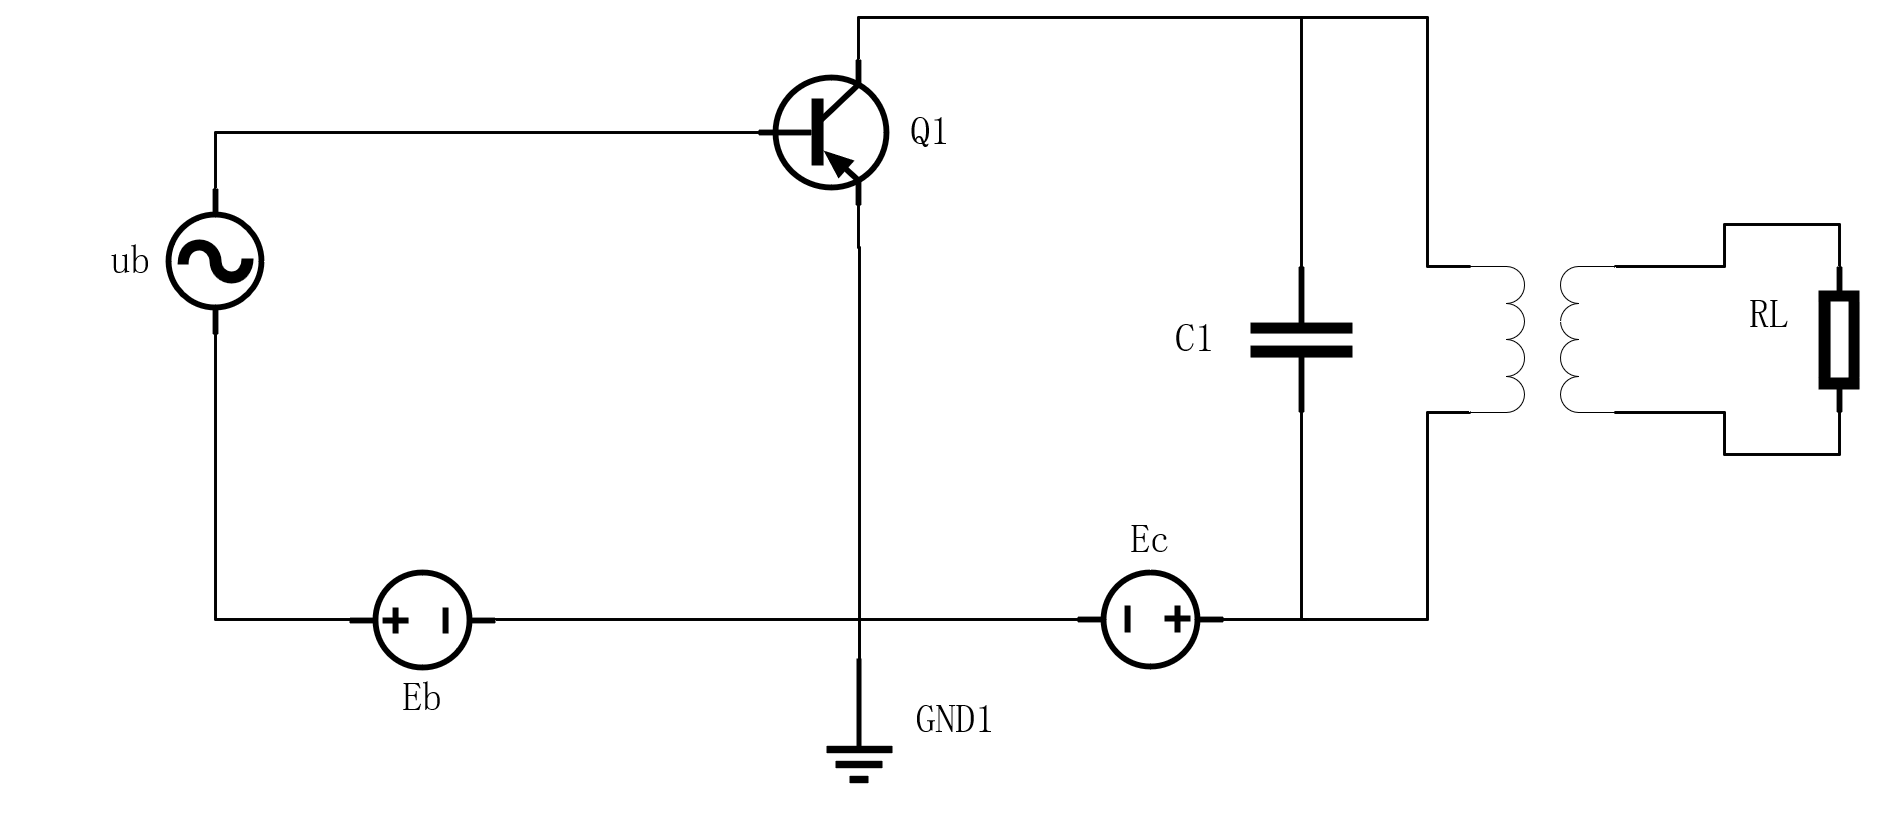
\includegraphics[width=0.8\textwidth]{Figure/谐振功率放大器电路图.png} 
       \caption{谐振功率放大器电路}
    \end{figure}

    基极偏置电压为$E_b$,交流信号为$u_b$，集电极电源为$E_c$

    \subsection{工作原理}
    采用丙类运放（为提高效率），得到的波形为图2的余弦脉冲函数，由傅里叶级数展开可知，一个周期函数可以由多个正弦量表达出来，而RLC并联谐振在谐振点$\omega_0$处阻抗最大（串联谐振最小）可以实现一个选频功能，从而得到想要的频率。
    \begin{figure}[h]
        \centering
        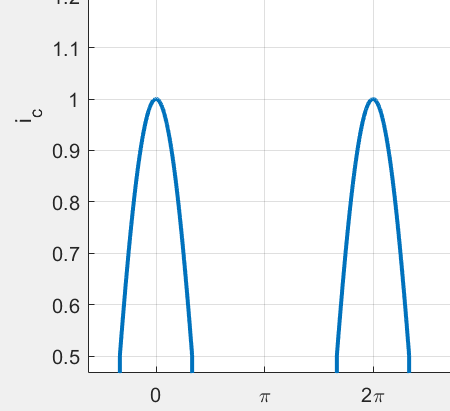
\includegraphics[width=0.5\textwidth]{Figure/余弦脉冲函数.png}
        \caption{余弦脉冲函数}
    \end{figure}
    \begin{equation}
        i_c=I_{C0}+i_c1+...+i_cn
    \end{equation}
    \begin{equation}
        i_c=I_C0+I_{c1m}cos\omega t+I_{c2m}cos2\omega t+....
    \end{equation}

    由式1-2可知，可以分解出直流分量$I_{C0}$和基次交流分量$cos\omega t$一直到$n$次分量$cosn\omega t$

    为什么丙类功放效率最高：当三极管导通时，电流通过时间越长发热越多效率越低

    \subsection{高频功率放大器中的能量关系}
    在集电极电路中，LC回路得到的高频功率$P_O$为
    \begin{equation}
        P_O=\frac{1}{2}I_{c1m}\cdot U_{cm}=\frac{1}{2}I^2_{c1m}\cdot R_e=\frac{1}{2}\frac{U^2_{cm}}{R_e}
    \end{equation}
    其中$R_e$为$LC$谐振回路的谐振电阻，$U_{cm}$为集电极输出电压的振幅

    集电极电源$E_C$供给的直流输入功率为:
    \begin{equation}
        P_E=E_C\cdot I_{C0}
    \end{equation}
    直流输入功率$P_E$，集电极输出高频功率$P_O$，集电极耗散功率$P_C$的关系
    \begin{equation}
        P_C=P_E-P_O
    \end{equation}
    集电极效率$\eta_c$为输出高频功率与直流输入功率之比
    \begin{equation}
        \eta_c=\frac{P_O}{P_E}=\frac{1}{2}\cdot\frac{I_{c1m\cdot U_{cm}}}{I_{C0}\cdot E_C}
    \end{equation}

    \newpage

    \subsection{丙类谐振功率放大器的工作状态分析}
        \subsubsection{解析分析法}
        \begin{figure}[h]
            \begin{minipage}{0.48\textwidth}
                \centering
                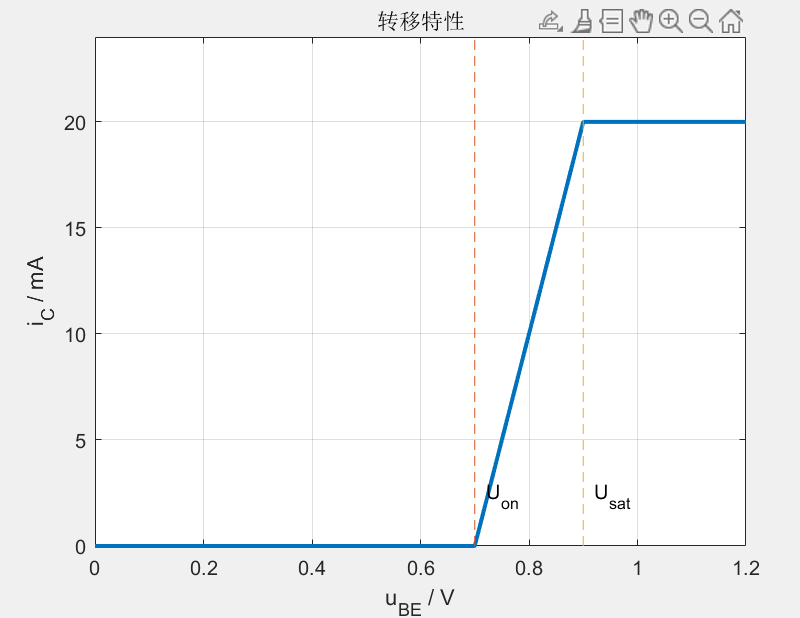
\includegraphics[width=0.8\textwidth]{Figure/转移特性.png}
                \caption{理想化的转移特性曲线}
            \end{minipage}
            \begin{minipage}{0.48\textwidth}
                \centering
                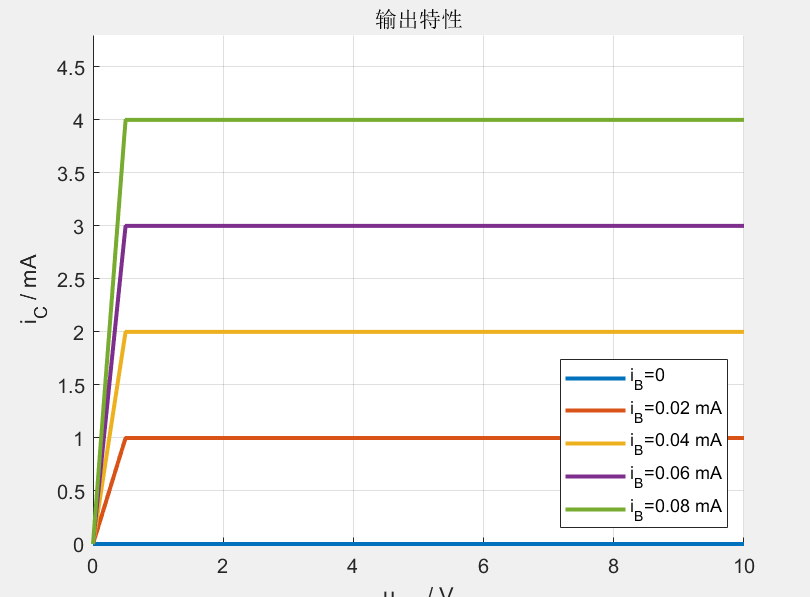
\includegraphics[width=0.8\textwidth]{Figure/输出特性.png}
                \caption{理想化的输出特性曲线}
            \end{minipage}
        \end{figure}
        转移特性曲线中$i_C=g_m(u_BE-U_B')$




\end{document}